\documentclass{beamer}

\usepackage{amsmath}
\usetheme{Marburg} 
\usepackage{graphicx}
\usepackage{color,listings}

\DeclareGraphicsExtensions{.png}


\lstset{language=java}
\lstset{breaklines=true}
\lstset{showstringspaces=false}
\lstset{tabsize=3}
\lstset{basicstyle=\ttfamily\scriptsize}
\lstset{breakautoindent=true}
\lstset{postbreak=\space}
\title{An Eclipse-based Integrated and Automated
Fault Localization System}
\author{Tristan Challener}
\date{\today}

\begin{document}
	\begin{frame}
	\titlepage
	\end{frame}
	
	%%%%%%%%%%%% Slide %%%%%%%%%%%%%%%%%%%%%%%%%%%%%%%%%%%%%%%%%%%%%%%%%%%
	\section{Contents}
	\begin{frame}
	\frametitle{Table of Contents}
	\begin{enumerate}
	  \item Motivation
	  \item Project Overview
	    \begin{enumerate}
	      \item Automatic Fault Localization
	      \item Empirical Study
	      \item CodeCover
	    \end{enumerate}
	  \item Feasibility
	    \begin{enumerate}
	      \item Using CodeCover
	      \item Parsing Output
	    \end{enumerate}
	  \item Conclusion
	\end{enumerate}
	\end{frame}
	%%%%%%%%%%%% Slide %%%%%%%%%%%%%%%%%%%%%%%%%%%%%%%%%%%%%%%%%%%%%%%%%%%
	\section{Motivation}
	\begin{frame}
	\frametitle{Motivation}
	\begin{itemize}
	  \item Debugging is complex and difficult
	    \pause
	  \item Fault localization is the most expensive
	    \pause
	  \item Current techniques insufficient
	\end{itemize}
	\end{frame}
	%%%%%%%%%%%% Slide %%%%%%%%%%%%%%%%%%%%%%%%%%%%%%%%%%%%%%%%%%%%%%%%%%%
	\section{Project Overview}
	\subsection{AFL}
	\begin{frame}
	\frametitle{Automatic Fault Localization}
	\begin{itemize}
	  \item Uses per-test coverage analysis
	    \pause
	  \item Ranks statements by suspiciousness
	    \pause
	  \item Variety of risk evaluation functions
	  \begin{equation*}
	suspiciousness(e) = 1 - \frac{\frac{failed(e)}{total failed}}{\frac{passed(e)}{total passed} + \frac{failed(e)}{total failed}}
	  \end{equation*}
	\end{itemize}
	\end{frame}
	%%%%%%%%%%%% Slide %%%%%%%%%%%%%%%%%%%%%%%%%%%%%%%%%%%%%%%%%%%%%%%%%%%
	\subsection{Empirical Study}
	\subsubsection{EXAM}
	\begin{frame}
	\frametitle{EXAM Score}
	\begin{itemize}
	   	\item One method for comparing risk evaluation functions
	   	\pause
	   	\item Ranking of faulty statement in suspiciousness
	   	\pause
	   	\item Percentage of statements not needed to consider
	   	\pause
	   	\item Higher-is-better metric
	\end{itemize}
	\end{frame}
	%%%%%%%%%%%% Slide %%%%%%%%%%%%%%%%%%%%%%%%%%%%%%%%%%%%%%%%%%%%%%%%%%%
	\begin{frame}
	\frametitle{EXAM Score}
	\begin{figure}
		\label{tareff}
		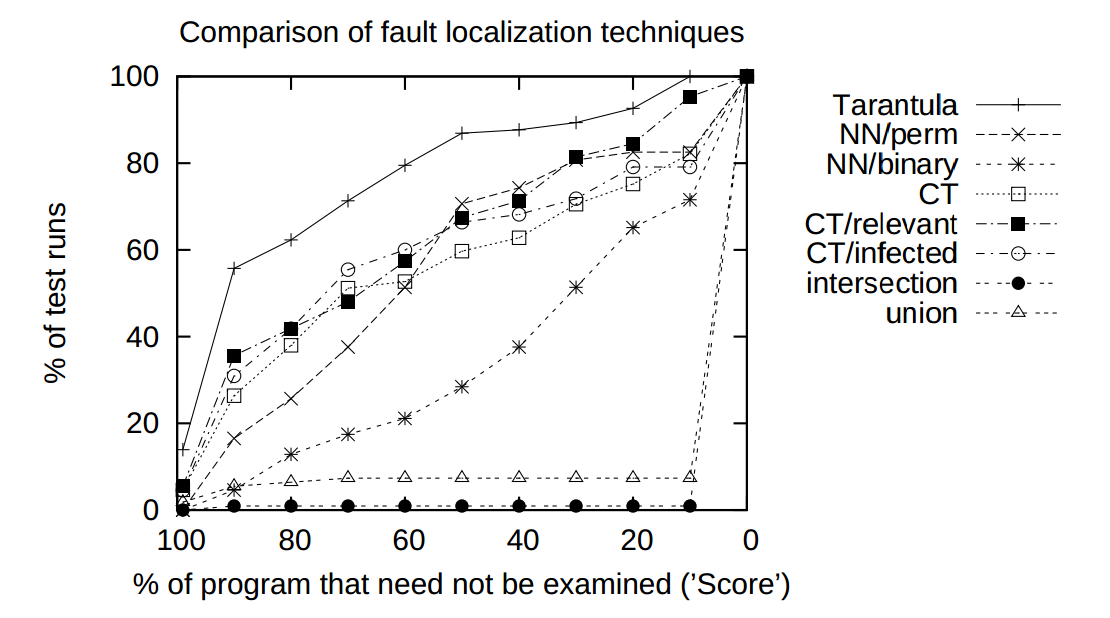
\includegraphics[width=4in]{img/tareff}
	\end{figure}
	\end{frame}
	%%%%%%%%%%%% Slide %%%%%%%%%%%%%%%%%%%%%%%%%%%%%%%%%%%%%%%%%%%%%%%%%%%
	\subsubsection{NCP}
	\begin{frame}
	\frametitle{NCP Score}
	\begin{itemize}
    	\item Alternate method for comparing risk evaluation functions
    	\pause
    	\item Risk evaluation function becomes heuristic for GenProg
    	\pause
    	\item Number of patches before correct patch
    	\pause
    	\item Lower-is-better metric
	\end{itemize}
	\end{frame}
	%%%%%%%%%%%% Slide %%%%%%%%%%%%%%%%%%%%%%%%%%%%%%%%%%%%%%%%%%%%%%%%%%%
	\begin{frame}
	\frametitle{NCP Score}
	  	\begin{figure}
	  		\label{ncpeval}
	  		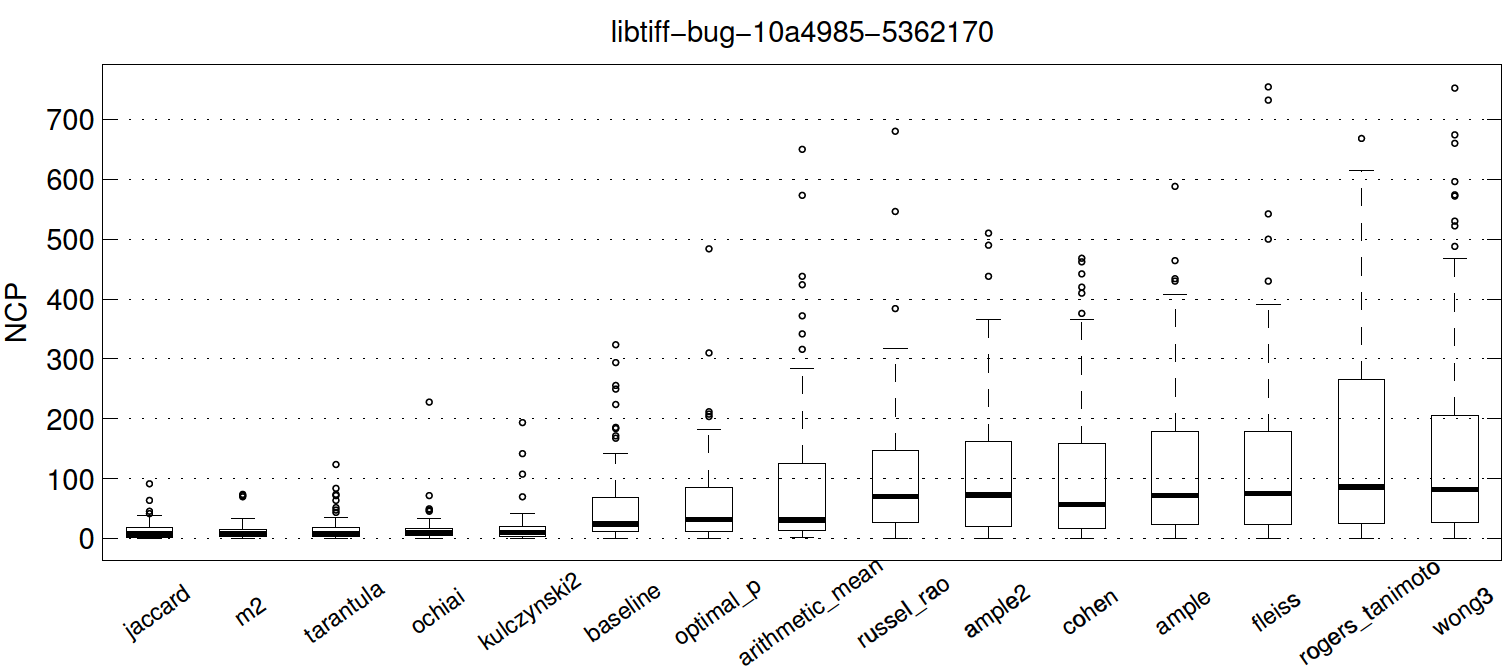
\includegraphics[width=4in]{img/ncpeval}
	  	\end{figure}
	\end{frame}
	%%%%%%%%%%%% Slide %%%%%%%%%%%%%%%%%%%%%%%%%%%%%%%%%%%%%%%%%%%%%%%%%%%
	\subsubsection{Empirical Study}
	\begin{frame}
	\frametitle{Empirical Study}
	\begin{itemize}
    	\item Use EXAM score to compare risk evaluation functions
    	\pause
    	\item Select from existing studies
    	\pause
    	\item GenProg(NCP) comparison
    	\pause
    	\item Theoretical comparison
	\end{itemize}
	\end{frame}
	%%%%%%%%%%%% Slide %%%%%%%%%%%%%%%%%%%%%%%%%%%%%%%%%%%%%%%%%%%%%%%%%%%
	\subsection{CodeCover}
	\begin{frame}
	\frametitle{CodeCover Coverage}
	\begin{itemize}
    	\item Eclipse-compatible coverage analysis tool
    	\pause
    	\item Uses existing JUnit test suites
    	\pause
    	\item Generates coverage information for each test method
    	\pause
    	\item Stores output in readable format (XML)
	\end{itemize}
	\end{frame}
	%%%%%%%%%%%% Slide %%%%%%%%%%%%%%%%%%%%%%%%%%%%%%%%%%%%%%%%%%%%%%%%%%%
	\section{Feasibility}
	\subsection{Using CodeCover}
	\begin{frame}
	\frametitle{Using CodeCover}
	\begin{itemize}
    	\item Tested with a simple existing system with a JUnit test suite
    	\pause
    	\item Successfully produced per-test coverage
    	\pause
    	\item Produced XML representation of coverage data
	\end{itemize}
	\end{frame}
	%%%%%%%%%%%% Slide %%%%%%%%%%%%%%%%%%%%%%%%%%%%%%%%%%%%%%%%%%%%%%%%%%%
	\begin{frame}
	\frametitle{Coverage Highlighting}
	  	\begin{figure}
	  		\label{coverage}
	  		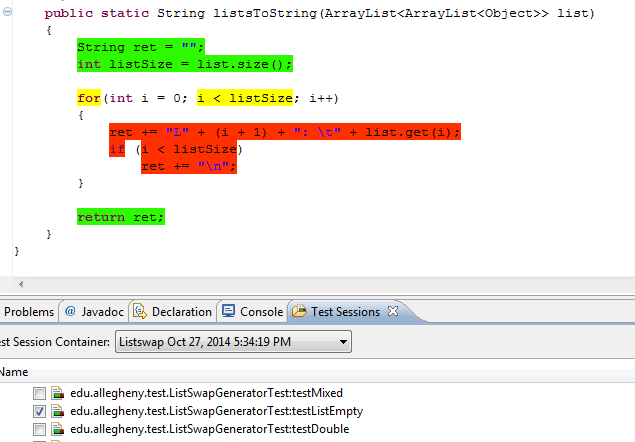
\includegraphics[width=3in]{img/codecovercoverage}
	  	\end{figure}
	\end{frame}
	%%%%%%%%%%%% Slide %%%%%%%%%%%%%%%%%%%%%%%%%%%%%%%%%%%%%%%%%%%%%%%%%%%
	\begin{frame}
	\frametitle{Per-test Coverage}
	  	\begin{figure}
	  		\label{ptcoverage}
	  		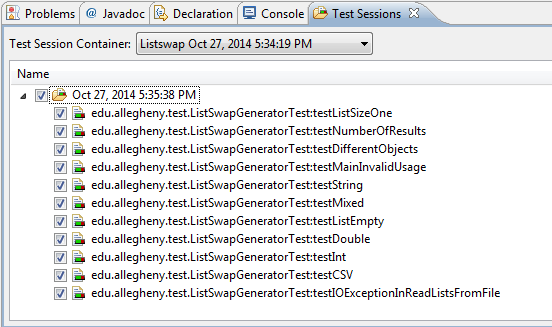
\includegraphics[width=3in]{img/codecoverpertest}
	  	\end{figure}
	\end{frame}
	%%%%%%%%%%%% Slide %%%%%%%%%%%%%%%%%%%%%%%%%%%%%%%%%%%%%%%%%%%%%%%%%%%
	\subsection{Parsing Output}
	\subsubsection{XML Representation}
	\begin{frame}
	\frametitle{XML Representation}
	\begin{itemize}
    	\item Contains several pieces of information:
    	\pause
    	\begin{itemize}
    		\item Complete source code
    		\item Statement definitions
    		\item List of statements covered by each test method for each file under test
    		\pause
    	\end{itemize}
	\end{itemize}
	\begin{figure}
		\label{xmlstat}
		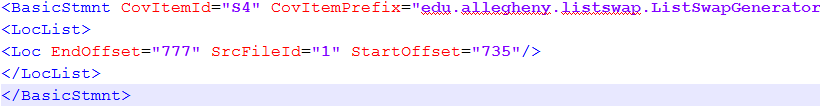
\includegraphics[width=4in]{img/xmlstatement}
	\end{figure}
	\end{frame}	
	%%%%%%%%%%%% Slide %%%%%%%%%%%%%%%%%%%%%%%%%%%%%%%%%%%%%%%%%%%%%%%%%%%
	\begin{frame}
	\frametitle{XML Representation}
	  	\begin{figure}
	  		\label{xmlcov}
	  		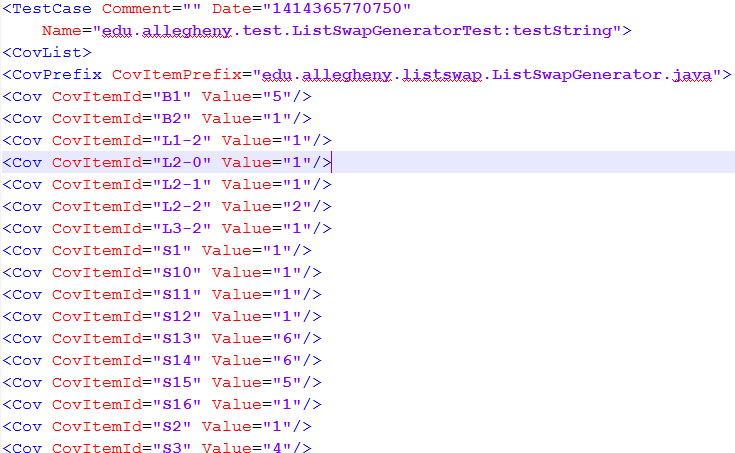
\includegraphics[width=4in]{img/xmlcoverage}
	  	\end{figure}
	\end{frame}
	%%%%%%%%%%%% Slide %%%%%%%%%%%%%%%%%%%%%%%%%%%%%%%%%%%%%%%%%%%%%%%%%%%
	\subsubsection{Parsing XML}
	\begin{frame}
		\frametitle{Parsing XML}
		\begin{itemize}
	    	\item Document Object Model(DOM) parsing
	    	\pause
	    	\item Translate entire XML document into Java tree structure
	    	\pause
	    	\item Allows ease of handling data once built
		\end{itemize}
	\end{frame}
	%%%%%%%%%%%% Slide %%%%%%%%%%%%%%%%%%%%%%%%%%%%%%%%%%%%%%%%%%%%%%%%%%%
	\begin{frame}
	\frametitle{Parsing XML}
	  	\begin{figure}
	  		\label{parsedxmlstmt}
	  		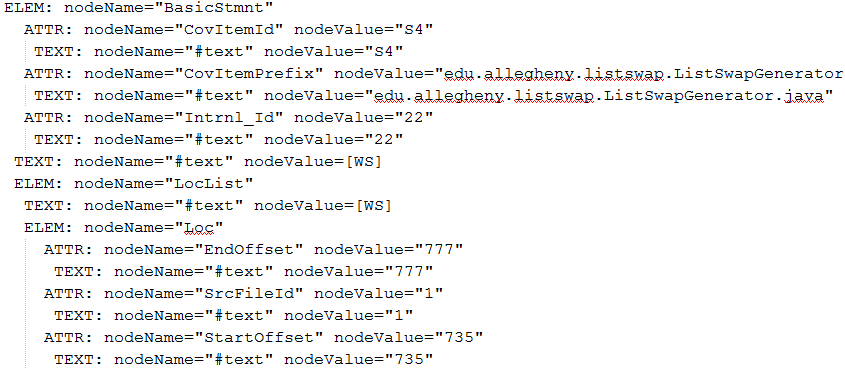
\includegraphics[width=4in]{img/parsedxmlstmt}
	  	\end{figure}
	\end{frame}
	%%%%%%%%%%%% Slide %%%%%%%%%%%%%%%%%%%%%%%%%%%%%%%%%%%%%%%%%%%%%%%%%%%
	\begin{frame}
	\frametitle{Parsing XML}
	  	\begin{figure}
	  		\label{parsedxmlcover}
	  		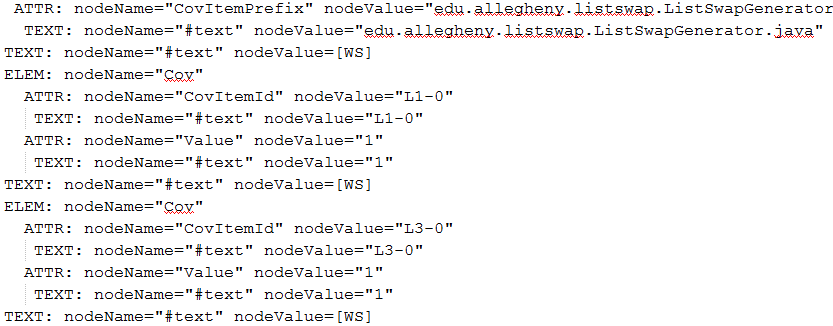
\includegraphics[width=4in]{img/parsedxmlcover}
	  	\end{figure}
	\end{frame}
	%%%%%%%%%%%% Slide %%%%%%%%%%%%%%%%%%%%%%%%%%%%%%%%%%%%%%%%%%%%%%%%%%%
	\section{Conclusion}
	\begin{frame}
		\frametitle{Conclusion}
		\begin{itemize}
	    	\item Create an Eclipse plugin that uses existing tools
	    	\pause
	    	\item Combine existing tools in a single fault localization system
	    	\pause
	    	\item Ambitious, but feasible
		\end{itemize}
	\end{frame}
	%%%%%%%%%%%% Slide %%%%%%%%%%%%%%%%%%%%%%%%%%%%%%%%%%%%%%%%%%%%%%%%%%%
	\section{References}
	\begin{frame}
	\frametitle{References}
	\tiny
	\vspace{0.2in}
	\bibliographystyle{plain}
	\bibliography{senior_thesis_proposal}
	\nocite{harrold}
	\nocite{genprog}
	\nocite{theory}
	\end{frame}
\end{document}
